%***************************************************************************
% MCLab Protocol Template
%
% Embedded Computing Systems Group
% Institute of Computer Engineering
% TU Vienna
%
%---------------------------------------------------------------------------
% Vers.	Author	Date	Changes
% 1.0	bw	10.3.06	first version
% 1.1	bw	25.4.06	listing is in a different directory
% 1.2	bw	24.5.06	tutor has to be listed on title page
% 1.3	bw	16.6.06	statement about no plagiarism on title page (sign it!)
%---------------------------------------------------------------------------
% Author names:
%       bw      Bettina Weiss
%***************************************************************************

\documentclass[12pt,a4paper,titlepage,oneside]{article}
\usepackage{graphicx}            		% fuer Bilder
\usepackage{epsfig}              		% fuer EPS Bilder
\usepackage{listings}            		% fuer Programmlistings
%\usepackage{german}              	% fuer deutsche Umbrueche
\usepackage[latin1]{inputenc}    	% fuer Umlaute
\usepackage{times}               		% PDF files look good on screen
\usepackage{amssymb,amsmath,amsthm}
\usepackage{dsfont}

%***************************************************************************
% SES: own packages
%***************************************************************************
\usepackage{color}				% color definitions
\usepackage{url}				% web urls
\usepackage[amssymb]{SIunits}	% common units
\usepackage{jurabib}			% bibliography support

%***************************************************************************
% note: the template is in English, but you can use German for your
% protocol as well; in that case, remove the comment from the
% \usepackage{german} line above
%***************************************************************************


%***************************************************************************
% enter your data into the following fields
%***************************************************************************
\newcommand{\Vorname}{Stefan}
\newcommand{\Nachname}{Seifried}
\newcommand{\MatrNr}{0925401}
\newcommand{\Email}{e0925401@student.tuwien.ac.at}
\newcommand{\Part}{I}
\newcommand{\Tutor}{Christoph Haderer}
%***************************************************************************


%***************************************************************************
% generating the document from Protocol.tex:
%       "latex Protocol"        generates a .dvi file
%       "latex Protocol"        repeat to get correct table of contents
%       "xdvi Protocol &"       shows the .dvi file on viewer
%       "dvips Protocol.dvi -o Protocol.ps"      generates a postscript file
%
%***************************************************************************

%---------------------------------------------------------------------------
% include all the stuff that is the same for all protocols and students
\input ProtocolHeader.tex
%---------------------------------------------------------------------------

\begin{document}

%***************************************************************************
% SES: set code formatting
%***************************************************************************
%---------------------------------------------------------------------------
% set custom color definitions
\definecolor{green}{rgb}{0.0,0.6,0.0}
%---------------------------------------------------------------------------

%---------------------------------------------------------------------------
% set code listing formatting
\lstset{language=C}
\lstset{frame=single}
\lstset{numbers=left}
\lstset{showspaces=false}
\lstset{showstringspaces=false}
\lstset{linewidth=\textwidth}
\lstset{commentstyle=\color{green}}
\lstset{keywordstyle=\color{blue}\bfseries}
\lstset{postbreak=\space, breakindent=5pt, breaklines}
%---------------------------------------------------------------------------

%---------------------------------------------------------------------------
% set paragraph formatting
\setlength{\parindent}{0pt} 
%---------------------------------------------------------------------------

%---------------------------------------------------------------------------
% set up bibliography
\jurabibsetup{
	commabeforerest,
	ibidem=strict,
	citefull=first,
	see,
	titleformat={colonsep,all},
}

\renewcommand*{\jbauthorfont}{\textsc}
\renewcommand*{\biblnfont}{\scshape\textbf}
\renewcommand*{\bibfnfont}{\normalfont\textbf}
%---------------------------------------------------------------------------

%---------------------------------------------------------------------------
% create titlepage and table of contents
\MakeTitleAndTOC
%---------------------------------------------------------------------------


%***************************************************************************
% This is where your protocol starts
%***************************************************************************

%***************************************************************************
\section{Overview}
%***************************************************************************

%---------------------------------------------------------------------------
\subsection{Connections}
%---------------------------------------------------------------------------

\bConnections{\SDIO}{}
PD4:6 & BTN1:3 \\
\BTNCOMa & GND \\
PA0 & P1 (TRIM1) \\
$\text{VCC}_{\text{IOBoard}}$ & $\text{VCC}_{\text{M16Board}}$ \\
$\text{GND}_{\text{IOBoard}}$ & $\text{GND}_{\text{M16Board}}$ \\
\eConnections

\bConnections{ \LCD}{}
PA4:7 & LCD\_DB4:7 \\
PA1 & LCD\_RS \\
PA2 & LCD\_RW \\
PA3 & LCD\_EN \\
\eConnections

\bConnections{\MPa}{}
PC0 & MOSI \\
PC1 & SCK \\
PC2 & MISO \\
PC3 & MMC\_CS \\
PC4 & MP3\_CS \\
PC5 & BSYNC \\
PC6 & MP3\_RESET \\
PC7 & MMC\_CD \\
PD2 & DREQ \\
$\text{VCC}_{\text{MP3}}$ &  $\text{VCC}_{\text{M16Board}}$ \\
$\text{GND}_{\text{MP3}}$ & $\text{GND}_{\text{M16Board}}$ \\
\eConnections

{ \bf PORTB } is left blank by intention since { \bf PB5, PB6, PB7 } most likely collide with the UART.  

%---------------------------------------------------------------------------
\subsection{Design Decisions}
%---------------------------------------------------------------------------

\begin{enumerate}
	\item I omitted the implementation of a SD-card CRC check regarding of two reasons. First one was the space of CRC16 lookup table, as I used in the {\it Boiler Control} application. Second thoughts that for mp3 playback it is sufficient that most bits are correct and that necessary retransmissions would hurt more.
	
	\item The size of an index file entry is limited to 64Byte (described in {\it Prepare an Image} section). Since this information is completely kept in RAM and there is no possibility to move this to Flash it tried it to keep it as small as possible. Therefore there are only 55 characters available for the storage of artist and title.
	 
\end{enumerate}

%---------------------------------------------------------------------------
\subsection{Specialities}
%---------------------------------------------------------------------------

Most noteable are the implementation of the CGRAM Character's for the LCD-Display, and the usage of a scheduler based architecture (described in {\it Main Application} section).


%***************************************************************************
\section{Main Application}
%***************************************************************************

The main application designed was inspired by the article {\it Get by without an RTOS } published in {\it Embedded System Programming}.\footcite{Embedded} Therefore I used a single {\bf 10 ms } timer that manages all background tasks. Basically I used three type of tasks:

\begin{enumerate}
	\item event driven tasks
	\item state machine tasks
	\item timed tasks
\end{enumerate}

{\bf event driven tasks:} This type uses a event queue implementation where other tasks can put predefined requests. The requests are processed in the same order as they arrive, although it would be easily possible to implement some kind of priority queue. One request is processed per time slice, if there are no requests pending it will continue immediately processing other tasks. A good example for this kind of task would be {\it task\_playercontrol}.

{\bf state machine tasks:} State machines can advance one state per time slice, so basically they most likely execute some code every time slice except there is an explicitly defined idle state. A good example is {\it task\_mmccard}, this module uses the state machine to watch the SD-Card port. Every time slice it tries to bring up the SD-Card, in case any error during SD-Card operations occur the state machine is put back to the very beginning.

{\bf timed tasks:} Those tasks are executed on an arbitrary multiple of the time slice. This value is defined in the {\bf Reload Value} of the task structure. Again a good example would be the {\it task\_keypad} module, which checks the input port for any changes to detect key presses.

The modules implementing this behaviour are {\it os\_task} and  {\it os\_scheduler}, where the last module is mainly responsible for execution control.

%***************************************************************************
\section{SPI Implementation}
%***************************************************************************

The SPI implementation is completely written in cross-assembler, which is a mixture of standard avr assembly and C Macro's. This has some advantages as you can stick to your habits, e.g. using the { \it \_BV } macro for bit shifting.

The SPI reaches a total speed of { \bf 8 clock cycles per bit }. Considering the microprocessor speed of { \bf 16 MHz } this makes up a decent frequency of { \bf 2 MHz } for the SPI. Although the effective data rate is a little bit slower because of the setup needed for the first byte sent and of course some stuff that is needed for cleanup. Considering an overhead per byte of about { \bf 25 clock cycles per byte } we are able to send a byte in about { \bf 90 clock cycles } resulting in an effective maximum data rate of about { \bf 1.5 MBit }.  As tested, this is more than sufficient to play the required 128KBit mp3 files.

This quite impressive data rate is reached with some assumptions and tricks presented in the lecture. Most noteable I made extensive use of { \it loop unrolling } in both the receive and the send functions. This saved me some valuable time omitting the increment/decrement of a counter and expensive jump instructions. I also preread the data port for the {\it send } function, instead of following the read/modify/write pattern. I considered this valid since I disabled any interrupts at start so the function is atomic. This allowed me to save a valuable clock cycle since the assembler commands for bit wise set/clear ({ \it sbi/cbi }) take both { \bf 2 clock cycles} and a { \it out } command takes only { \bf 1 clock cycle}. 

According to the mp3 decoder datasheet \footcite[22]{VS1011} it expects SPI {\it mode 1}, this means a clock polarity 0 and a clock phase of 1. There was also an implementation with {\it mode 0} since this was suggested to be most compatible with the SD-Card, but was removed since it worked out fine with the { \it mode 1} implementation. In {\it figure 1} and {\it figure 2} you see timing diagrams for all four modes used for implementing the SPI driver. \footcite[11]{AVRSPI}

\begin{figure}[htbp]
	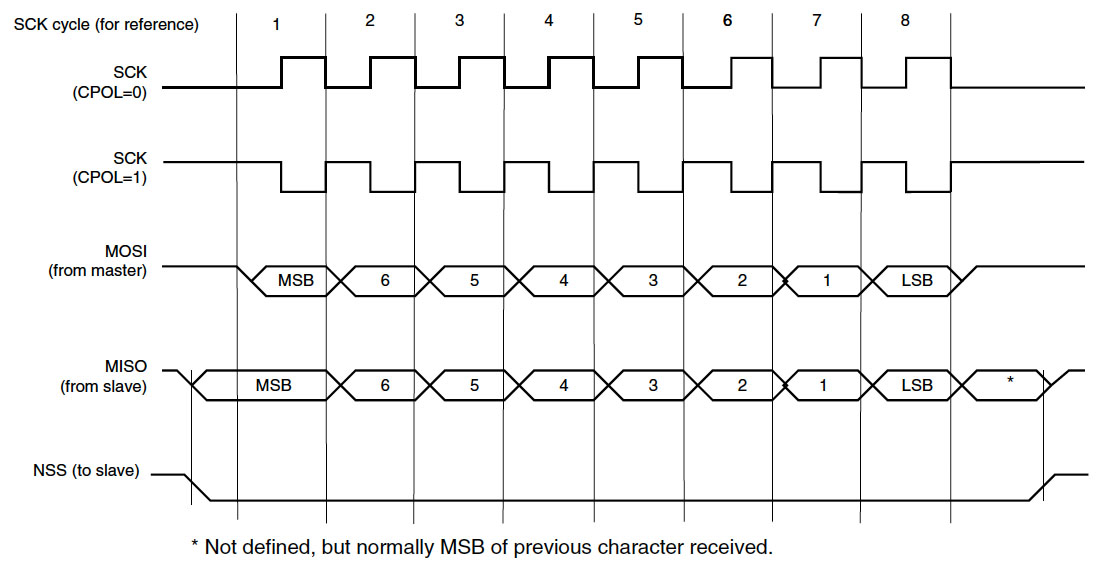
\includegraphics[width=1.0\textwidth]{ressources/spi_phase_1}
	\caption{SPI Transfer Format Phase '1'}
\end{figure}

\begin{figure}[htbp]
	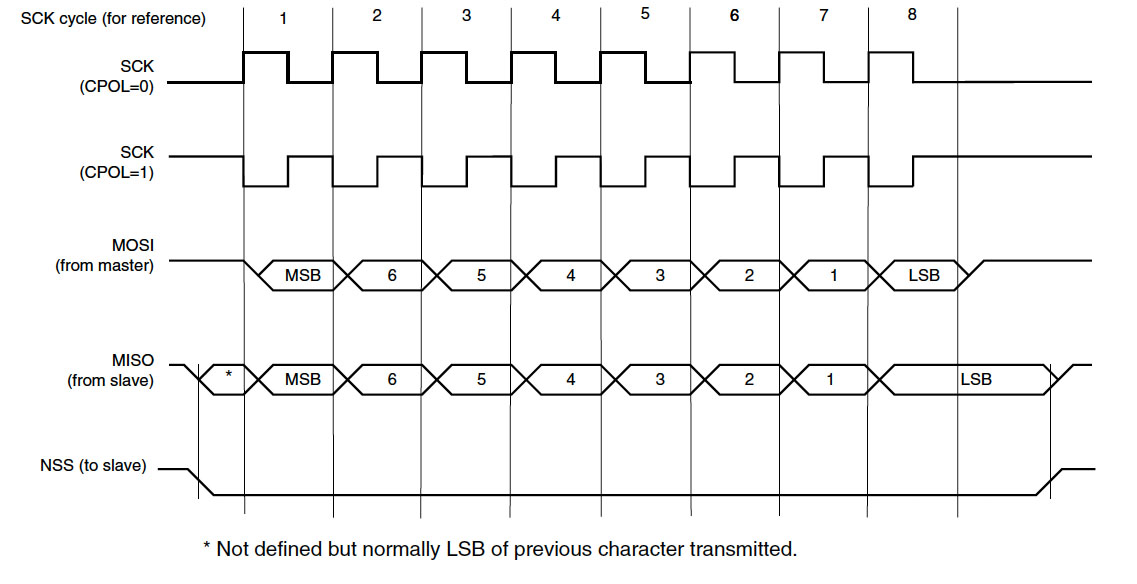
\includegraphics[width=1.0\textwidth]{ressources/spi_phase_0}
	\caption{SPI Transfer Format Phase '0'}
\end{figure}

%***************************************************************************
\section{File System}
%***************************************************************************

FAT16 was chosen as file system, since Microsoft published a full specification document during it's Extensible Firmware Interface offensive back in 2000.\footcite{FAT16}. I found no way to reduce most of the expensive 32bit operations without sacrificing any flexibility. E.g. on the web there are lots of implementations that assume the sector size is 512 bytes, although there are are plenty of other sector sizes that are valid. There would have been two things, that I didn't implement due to increased memory usage but I thought would increase performance drastically:

\begin{enumerate}
	\item buffering some cluster addresses, e.g. 16, so the driver could read a larger data area before looking at the file allocation table again.
	\item increase the read size to the sector size. This would have the advantage of not needing any sector offset calculation, unfortunately this would be far beyound the limits of the microcontroller  
\end{enumerate}

The implementation itself is pretty much modeled after stream based io operations in C. Therefore there is a {\bf 'open', 'read' and 'seek' - operation}, apart from the stuff needed to do address calculation.

In order to prevent parsing any id3 tags from the file a {\bf 64 byte} aligned file was used as index data. This file contains the necessary meta information for the mp3 player to find mp3 files and display the artist and title information accordingly. The detailed specifications and how to prepare an image are discussed in the { \it image creation section}. The mp3 files themselves can simply be drag and dropped from your PC and no further special preparations are needed. 

%***************************************************************************
\section{MP3 Decoder}
%***************************************************************************

The mp3 decoder uses the external interrupt {\bf INT0} for data flow control during mp3 playback. Some commands therefore explicitly disable the interrupt flag to execute their code. E.g. the volume command must be atomic, since it is most likely also executed during mp3 playback and can be interrupted by a data request from the mp3 decoder chip.

Some of the functionality also makes use of the {\it coroutine pattern}\footcite{Knuth}, where state machines are used to allow basically non-interruptable parallel execution. This is useful to execute meaningful code while waiting for an event to happen.

%***************************************************************************
\section{Serial Interface}
%***************************************************************************

%---------------------------------------------------------------------------
\subsection{UART}
%---------------------------------------------------------------------------

The UART implementation is the same as already used for the boiler control application. But it now uses {\bf 38400,N,8,1} as connection parameters, which does a slight performance improve since sending is much faster now and a lot more stuff can be done during the time between the cycles serving the mp3 decoder.

Especially I, again, use output redirection to utilize stdio functionality provided by the C library.

%---------------------------------------------------------------------------
\subsection{Parser}
%---------------------------------------------------------------------------

Since all parser commands are of {\bf length 1} no special treatment was needed. The implementation is a simple state-machine like construct that handles single defined key-stroke. One speciality that is not mentioned in the specification is that the sine-test can be triggered by pressing the {\bf 'S'} key.

%---------------------------------------------------------------------------
\subsection{ANSI Terminal Emulation}
%---------------------------------------------------------------------------

In order to meet the specification required display via uart a basic implementation of a { \it VT100 ANSI Terminal } was needed, originally specified by Digital Equipment Corporation back in the 1970's. The standard is well known throughout the web\footcite{VT100}, so only some special character sequences were needed to fulfill the demanded functionality. The implementation was tested with { \it GTK-Term}, so the functionality may not be correct in other terminal emulations. E.g. I noticed during development, that { \it GTK-Term } itself did  not implement the terminal emulation correct, since it clearly stated that a {\it clear screen command } should send the cursor to the upper left corner which it does not in {\it GTK-Term}.

%***************************************************************************
\section{Buttons}
%***************************************************************************

All three buttons used by the application are not debounced by hardware. I used a simple counting algorithm for debouncing. Therefore after a state change has been detected it has to be stable for at least {\bf 4 scheduler time slices} (40 ms for used 10ms scheduler). 

In order to use minimum ressources for counting the stable slices I used the concept of {\it vertical counters}\footcite{Debounce} which implement counter's using clever bit tricks. Below you see the state diagram of 2 bits:

\begin{tabular}{|l|l|l|c|}
\hline
\textsc{present state} & \textsc{next state} \\
\textsc{A B} & { A B } \\
\hline
0 0 & 0 1 \\
0 1 & 1 0 \\
1 0 & 1 1 \\
1 1 & 0 0 \\ 
\hline
\end{tabular}

from this table we can derive two simple logic formulars to advance the counters.

\begin{equation}
\begin{aligned}
A = A \oplus B \\
B = \neg B
\end{aligned}
\end{equation}

using a state change as mask will then ensure that only counters advance where there is a state changed detected. This technique is extremely elegant and would allow up to 8 debounced inputs with a bare minimum memory and processor usage.

%***************************************************************************
\section{Volume Control}
%***************************************************************************

An 8-bit ADC is used for volume control, since volume control does not need to be that fine grained. It also seemed sufficient to poll the ADC only every {\bf 500 ms }, although this can be easily changed by modifying the {\it task reload value}. The ADC value is then inverted and shifted to the higher 8 Bits because the mp3 decoder expects a 16 Bit value and uses it as attenuation not gain. 

%***************************************************************************
\section{Resume Logic}
%***************************************************************************

The first time after a power outage the implementation tries to recover the previously played song. Therefore it saves the resume information to eeprom every time a new song is about to be played. If the song is not found, the first song is played. In order for a song recognized to be equivalent to the one stored in the resume information, both the file name and the title information have to be exact the same. This means also that it is possible that if you unplug the power change the sd-card, with the same song stored, it will also play the stored song. This could be circumvented by calculating some kind of checksum (crc, md5, \dots ).

Another interesting approach to keep eeprom writes to a minimum, would be the usage of the internal ADC Comparator connecting its input to an internal reference voltage. Therefore it would be possible to sense any upcoming supply voltage weakness, triggering an interrupt and writing the information to eeprom. This would be much better and elegant approach, but again I doubted this will work with the mc16 controller board due to the small capacitors and amount of peripheral devices that are connected.

%***************************************************************************
\section{Prepare an Image}
%***************************************************************************

In order to quickly prepare a test image I provided some scripts. Below you will find step by step instructions how to create a valid image:

\begin{enumerate}
	\item copy your mp3 files to folder {\it ./img/mp3/original}
	\item run {\it ./convert\_128k.sh} to convert your mp3 files to the required 128KBit/s Bitrate. The converted files are put in the folder {\it ./img/mp3/128k}.
	\item run {\it ./createid3info.sh ./128k} to create an {\it id3info.txt} index file.
	\item run {\it ./img/createimage\_128k.sh} which creates a SD-card image named {\it image\_128k.bin}
\end{enumerate}

Some specialities you may have noted:

{\bf File Naming:} The conversion script renames your mp3 files to {\bf 1.mp3, 2.mp3, 3.mp3, ...}. This is mostly due to the fact that I didn't find a way to generate the correct 8.3 naming in Linux for my {\it id3info.txt} index data. At the microcontroller I mostly rely on the 8.3 file name to determine which tag info corresponds to which file.

{\bf ID3INFO.TXT file format:} This file contains the artist and title information for the files, which omits the task of implementing a working id3 tag reader at the microcontroller. All lines must be {\bf 64 Byte aligned}, where the first {\bf 8 Bytes } are the file name, the next {\bf 55 Bytes } are artist and title information, and the last {\bf 1 Byte} is a line feed character. The microcontroller explicit checks that the file has at least one entry, therefore the file size must be at least 64 Bytes and that the file size is a multiple of 64 Bytes. I chose 64 Bytes as entry size, because this can be easily loaded with two read operations of the SD-card driver and should give sufficient space for most song titles and artists. For your convenience it is quite easy to modify the code to support larger entries.

%***************************************************************************
\section{Problems}
%***************************************************************************

The problem that caused most time, was that the mmc card rejected the second read command in case no communication took place for a longer period. Maybe this is also caused by the slow sector reading of the first 1-2 MBs. This could be solved by sending a few dummy packages via SPI that allowed the SD-card logic to wake up. With that little fix most SD-Card worked fine. Since this seems a common problem upon my colleagues I considered this a hardware/driver problem and did not further investigate this issue. 

%***************************************************************************
\section{Work}
%***************************************************************************

\begin{tabular}{|l|c|}
\hline
reading manuals, datasheets	& 8 h	\\
program design			& 12 h\\
programming				& 38 h\\
debugging				& 24 h\\
questions, protocol			& 20.0 h\\
image generation application   & 8 h \\
\hline
{\bf Total}					& 110.0 h \\
\hline
\end{tabular}



%***************************************************************************
\section{Theory Tasks}
%***************************************************************************

\QuText{
\textbf{[2 Points] Bitrate and Buffer:}} Consider the setup as
     described in the application specification where data is read in
     packets of 32Byte via SPI from an SD--Card by a microcontroller
     and afterwards written by SPI to a MP3 decoder chip.

Now assume the following:
\begin{enumerate}
\item The SPI is operated with a bitrate of $\mathit{BAUD}_{SPI}$
\item When reading from the SD--Card there is a overhead for SD--Card
     handling which reduces the bitrate of the SPI user data transfer
     by a factor of $\mathit{OVH}_{SD}$ where $1 \le \mathit{OVH}_{SD}$.
For example, $\mathit{OVH}_{SD}=1.2$ means that, if normally a some data needs
     time $X$ to be transfered via SPI, it needs time $1.2\times X$ to be
     read from the SD--Card.
\item The microcontroller needs time $t_s$ to switch the SPI from the
     SD--Card to the decoder chip and vice versa.
\item The microcontroller reads/writes 32Bytes before switching the SPI.
\item If the MP3 file is encoded with 128kBit/sec the decoder chip
     needs at least 128kbit/sec\footnote{We assume hereby that
     128kBit/sec = 128000Bit/sec.} of data to continuously play the
     file (this in fact means that we do not bother about the internal
     structure of the MP3 file).




\end{enumerate}


Based on the above, (1) derive a formula\footnote{Note, that it is not
     sufficient to only state the formula.
You really have to explain how you got to the result!} which,
     depending on the MP3 decoding, the SD overhead, and the switching
     time, gives the bitrate the SPI implementation has to guarantee.
Additionally, calculate the bitrate for the playback of a 128kBit/sec
     MP3, assuming an SD--card overhead of $1.5$ and a switching time
     of $10\mu s$.

(2) Given an SPI bitrate $\mathit{BAUD}_{SPI}^{*}>\mathit{BAUD}_{SPI}$
     and a internal buffer size of $\mathit{Buf}$.
Derive a formula how much 32Byte transfers of the above kind can be
     done until the buffer of the MP3 decoder chip is full (the DREQ
     pin goes low).
Additionally, calculate the number of transfers if
     $\mathit{BAUD}_{SPI}^{*}=400$kBit/sec and  $\mathit{Buf} =
     700$Bytes.

{\bf Solution (1):}

Let us define the following terms:

\begin{equation}
\begin{aligned}
T_{MP3} = \frac{1}{BAUD_{MP3}} \\
T_{SDCARD} = \frac{OVH_{SD}}{BAUD_{SPI}} \\
T_{SPI} = \frac{1}{BAUD_{SPI}}
\end{aligned}
\end{equation}

Therefore the timer needed for one mp3 bit ${\mathit T_{MP3}}$ is computed as follows:

\begin{equation}
T_{MP3} = T_{SDCARD} + \frac{t_s}{256} + T_{SPI} 
\end{equation}

Just insert the previous defined terms and rearrange to ${ \mathit BAUD_{SPI}}$

\begin{equation}
\begin{aligned}
\frac{1}{BAUD_{MP3}} = \frac{OVH_{SD}}{BAUD_{SPI}} + \frac{t_s}{256} + \frac{1}{BAUD_{SPI}} \\
\frac{1}{BAUD_{MP3}} - \frac{t_s}{256} = \frac{OVH_{SD}}{BAUD_{SPI}} + \frac{1}{BAUD_{SPI}} \\
BAUD_{SPI}*( \frac{1}{BAUD_{MP3}} - \frac{t_s}{256} ) = OVH_{SD} + 1 \\
BAUD_{SPI} = \frac{OVH_{SD} + 1}{ \frac{1}{BAUD_{MP3}} - \frac{t_s}{256} } \\
BAUD_{SPI} = \frac{ BAUD_{MP3}*256*(OVH_{SD} + 1) }{ 256 - t_s*BAUD_{MP3} }
\end{aligned}
\end{equation}

Insert the given values

\begin{equation}
\begin{aligned}
BAUD_{SPI} = \frac{ 128*10^3*256*(1.5 + 1) }{ 256 - 10^{-5}*128*10^3 } \\
BAUD_{SPI} = \frac{ 8.192*10^7 }{ 254.72 } \\
BAUD_{SPI} = \unit{321608}{bit/\second}
\end{aligned}
\end{equation}

{\bf Solution (2):}

The buffer is filled by the difference of $\mathit{BAUD}_{SPI}^{*}$ and $\mathit{BAUD}_{SPI}$

\begin{equation}
BAUD_{DIFF} = {BAUD}_{SPI}^{*} - BAUD_{SPI}
\end{equation}

From this we can compute the time necessary to fill the buffer

\begin{equation}
T_{BufferFull} = \frac{Buf*8}{BAUD_{DIFF}} 
\end{equation}

Multiplying this value with the original  $\mathit{BAUD}_{SPI}^{*}$ and alining this value to \unit{32}{Byte} we get the number of transfers

\begin{equation}
\begin{aligned}
N_{Transfers} = \frac{T_{BufferFull}* {BAUD}_{SPI}^{*}}{256} \\
N_{Transfers} = \frac{ \frac{Buf*8}{{BAUD}_{SPI}^{*} - BAUD_{SPI}}* {BAUD}_{SPI}^{*}}{256} \\
N_{Transfers} = \frac{ {BAUD}_{SPI}^{*} * Buf }{32*({BAUD}_{SPI}^{*} -  BAUD_{SPI})}
\end{aligned}
\end{equation}

Insert the given values


\begin{equation}
\begin{aligned}
N_{Transfers} = \frac{ 400*10^3 * 700 }{32*(400*10^3 -  321.6*10^3)} \\
N_{Transfers} \approx 112
\end{aligned}
\end{equation}

\QuText{
\textbf{[1 Points] Fibonacci warmup:}}  Prove that the series
     $a_1 = a_2 = 1$, and $a_n = a_{n-1}+a_{n-2}$, for $n\ge 2$, has
     the interesting property, that exactly every third element in the
     series is even.
Give a detailed, formal proof.

Hint: Prove by induction (with induction begin $a_1, a_2, a_3$,
     hypothesis, and step).

{\bf Solution:}

{\bf Basis:}

\begin{equation}
\begin{aligned}
a_3 = a_2 + a_1 = 1 + 1 = 2 \\
a_4 = a_3 + a_2 = 1 + 2 = 3 \\
a_5 = a_4 + a_3 = 2 + 3 = 5 \\
a_6 = a_5 + a_4 = 5 + 3 = 8 \\
\text{and so on \dots}
\end{aligned}
\end{equation}

{\bf Hypothesis:}

\begin{equation}
a_{3n} = 2m \text{ for } n \ge 2 
\end{equation}

{\bf Inductive Step:}

\begin{equation}
\begin{aligned}
a_{3(n+1)} = a_{3n+3}\\
 = a_{3n+2} + a_{3n+1}\\
 = a_{3n+1} + a_{3n} + a_{3n+1}\\
 = 2a_{3n+1}+a_{3n}\\
 = 2a_{3n+1} + 2m\\
 = 2(a_{3n+1} + m)
\end{aligned}
\end{equation}

As we see the hypothesis holds the prove as we still get a number multiplied by two, which is always even.

\QuText{
\textbf{[2 Points] Fibonacci File Names:}} Student Leonardo
     decided to implement the MP3-player's file system in the
     following way: he uses
     $\text{FAT}^\infty$,\footnote{$\text{FAT}^\infty$ is a very
     special imaginary implementation of FAT where filenames can get
     arbitrary long without exceeding the memory.} and MP3s have names
     of the form $n$.mp3, where $n \in \mathds{N}$, specifying the
     order in which the MP3s are to play.
Since he is short in time, he decides not to support more than the
     required $8$ MP3s.
However, as he loves math, he decides not to name them $0$.mp3,
     $1$.mp3, $2$.mp3, \dots, $7$.mp3 but does the following:   

Leonardo considers the same series $a_1, a_2, \dots$ as in the
     exercise above.
The file that is to play as the $k$th song, $0\le k\le 7$, is called
     $n$.mp3, where $n$ is the smallest number greater than $0$ that
     fulfills $a_n \pmod 8 = k$.

After some minutes he comes up with: $6$.mp3 is to play first since
     $a_6 \pmod 8 =  8 \pmod 8 = 0$, $1$.mp3 is to play second since
     $a_1 \pmod 8 = 1 \pmod 8 = 1$, $3$.mp3 is to play third since
     $a_3 \pmod 8 = 2 \pmod 8 = 2$, and $4$.mp3 is to play fourth
     since $a_4 \pmod 8 = 3 \pmod 8 = 3$.
Then he stops, and does not know how to proceed.

Show that Leonardo cannot complete his list by formally proving that
     there is no number $n$ such that $a_n \pmod 8 = 4$.

Hint: Again give a proof by induction but this time take
     $a_1,\dots,a_6$ as induction begin and consider the divisibility
     of the series elements.

{\bf Solution:}

At first step we define the recursive Fibonacci formula in the residue class ring $\mathbb{Z}/8\mathbb{Z} = \{0,1,2,3,4,5,6,7\}$.

\begin{equation}
a_n = a_{n-1} + a_{n-2} \text{ for } n \ge 2 \text{ in } \mathbb{Z}/8\mathbb{Z}
\end{equation}

therefore we need to prove that

\begin{equation}
4 \neq a_{n-1} + a_{n-2} \text{ in } \mathbb{Z}/8\mathbb{Z}
\end{equation}


we also know that a residue class ring must be periodic due to its nature as ring, and we also know that if we find the same number pair again we have also found the period. Concluding $(a_{r-1}, a_{r-2}) = (a_{s-1}, a_{s-2})$ and $r \neq s$

\begin{equation}
\begin{aligned}
a_3=a_2+a_1=1+1=2\\
a_4=a_3+a_2=1+2=3\\
a_5=a_4+a_3=3+2=5\\
a_6=a_5+a_4=5+3=0\\
a_7=a_6+a_7=0+5=5\\
a_8=a_7+a_6=5+5=2\\
a_9=a_8+a_7=2+5=7\\
a_10=a_9+a_8=7+2=1\\
a_11=a_10+a_9=1+7=0\\
a_12=a_11+a_10=0+1=1\\
a_13=a_12+a_11=1+1=2\\
\dots
\end{aligned}
\end{equation}

the value pairs $(a_{12}, a_{11}) = (a_1, a_2)$, therefore we have found the period and did not encounter $4$, which already proves that $4$ cannot be used by Leonardo.

{Remarks:}
I desperately tried to follow the hint in the specification, but could not find any property which I could contradict by induction and excluding only $4$. But I would be very interested to see it, so if it could be published after on the course homepage I would be very thankful.

%***************************************************************************
\newpage
\appendix
\section{Listings}
\small{
%***************************************************************************

%---------------------------------------------------------------------------
\subsection{SPI}
%---------------------------------------------------------------------------

\lstinputlisting{../src/asm_spi.h}
\lstinputlisting{../src/asm_spi.s}

%---------------------------------------------------------------------------
\subsection{Uart}
%---------------------------------------------------------------------------

\lstinputlisting{../src/usart.h}
\lstinputlisting{../src/usart.c}
\lstinputlisting{../src/usart_stdout.h}
\lstinputlisting{../src/usart_stdout.c}
\lstinputlisting{../src/task_usart.h}
\lstinputlisting{../src/task_usart.c}

%---------------------------------------------------------------------------
\subsection{Architecture}
%---------------------------------------------------------------------------

\lstinputlisting{../src/event_decoder.h}
\lstinputlisting{../src/event_decoder.c}
\lstinputlisting{../src/event_display.h}
\lstinputlisting{../src/event_display.c}
\lstinputlisting{../src/event_userio.h}
\lstinputlisting{../src/event_userio.c}
\lstinputlisting{../src/main.h}
\lstinputlisting{../src/main.c}
\lstinputlisting{../src/os_scheduler.h}
\lstinputlisting{../src/os_scheduler.c}
\lstinputlisting{../src/os_task.h}
\lstinputlisting{../src/task_playercontrol.h}
\lstinputlisting{../src/task_playercontrol.c}

%---------------------------------------------------------------------------
\subsection{File System/SD Card}
%---------------------------------------------------------------------------

\lstinputlisting{../src/fat.h}
\lstinputlisting{../src/fat.c}
\lstinputlisting{../src/mmc_driver.h}
\lstinputlisting{../src/mmc_driver.c}
\lstinputlisting{../src/task_mmccard.h}
\lstinputlisting{../src/task_mmccard.c}

%---------------------------------------------------------------------------
\subsection{MP3 Decoder}
%---------------------------------------------------------------------------

\lstinputlisting{../src/mp3decoder.h}
\lstinputlisting{../src/mp3decoder.c}
\lstinputlisting{../src/task_mp3decoder.h}
\lstinputlisting{../src/task_mp3decoder.c}

%---------------------------------------------------------------------------
\subsection{Volume Control}
%---------------------------------------------------------------------------

\lstinputlisting{../src/task_adc.h}
\lstinputlisting{../src/task_adc.c}

%---------------------------------------------------------------------------
\subsection{Keys}
%---------------------------------------------------------------------------

\lstinputlisting{../src/task_keypad.h}
\lstinputlisting{../src/task_keypad.c}

%---------------------------------------------------------------------------
\subsection{LCD}
%---------------------------------------------------------------------------

\lstinputlisting{../src/lcd.h}
\lstinputlisting{../src/lcd.c}
\lstinputlisting{../src/task_display.h}
\lstinputlisting{../src/task_display.c}

%---------------------------------------------------------------------------
\subsection{Misc}
%---------------------------------------------------------------------------

\lstinputlisting{../src/common.h}
\lstinputlisting{../src/stringman.h}
\lstinputlisting{../src/stringman.c}
\lstinputlisting{../src/stringtable.h}
\lstinputlisting{../src/stringtable.c}

%***************************************************************************
}% small

%---------------------------------------------------------------------------
% BibTex support
\bibliography{protocol}
\bibliographystyle{jurabib} 
%---------------------------------------------------------------------------

\end{document}

